\section{Background}
\label{S:Back}

\subsection{State of the Art}
\label{SS:Back:SOA}
    
In the literature there are two problems that are often addressed when dealing with MRSLAM:
\begin{enumerate}
\item robot coordination, i.e., how to cover the most area given an unknown environment \cite{julia2012comparison}, and
\item merging the data to create one global map posterior, which is what we will focus on.
\end{enumerate}

In the case where all relative robot poses are known, merging maps is a trivial problem using small modifications to existing SLAM techniques \cite{thrun2001probabilistic}. In the general MRSLAM problem, however, robots may start with unknown absolute and relative poses, and therefore merging of maps requires the discovery of relative relationships between different robot trajectories to build a single map. This is often a costly process, which in general can be solved for robots sharing a search space by estimating each robot's relative pose given a partial map, but this leads to exponential complexity with respect to the number of exploring robots \cite{fox2006distributed}. Nevertheless, several practical algorithms exist to circumvent this naive and inefficient approach,  including coarse topological matching and stitching techniques borrowed from computer vision \cite{birk2006merging}.


A majority of the papers employ a Rao-Blackwellized particle filter (RBPF) for building occupancy grids.  


\cite{howard2006multi,birk2006merging,lazaro2013multi,lee2012probabilistic}


-What does the literature cover?

-Where did it begin, what did it progress to?




\subsection{\cite{howard2006multi} Extension to Original Work}
\label{SS:Back:Contributions}

\[
w_3^i=w_2^i w_1^i
\]


\begin{figure}[h]
\centering
\subfigure[Case where the peak weights are chosen, instead only mediocre points get the highest weighting.]{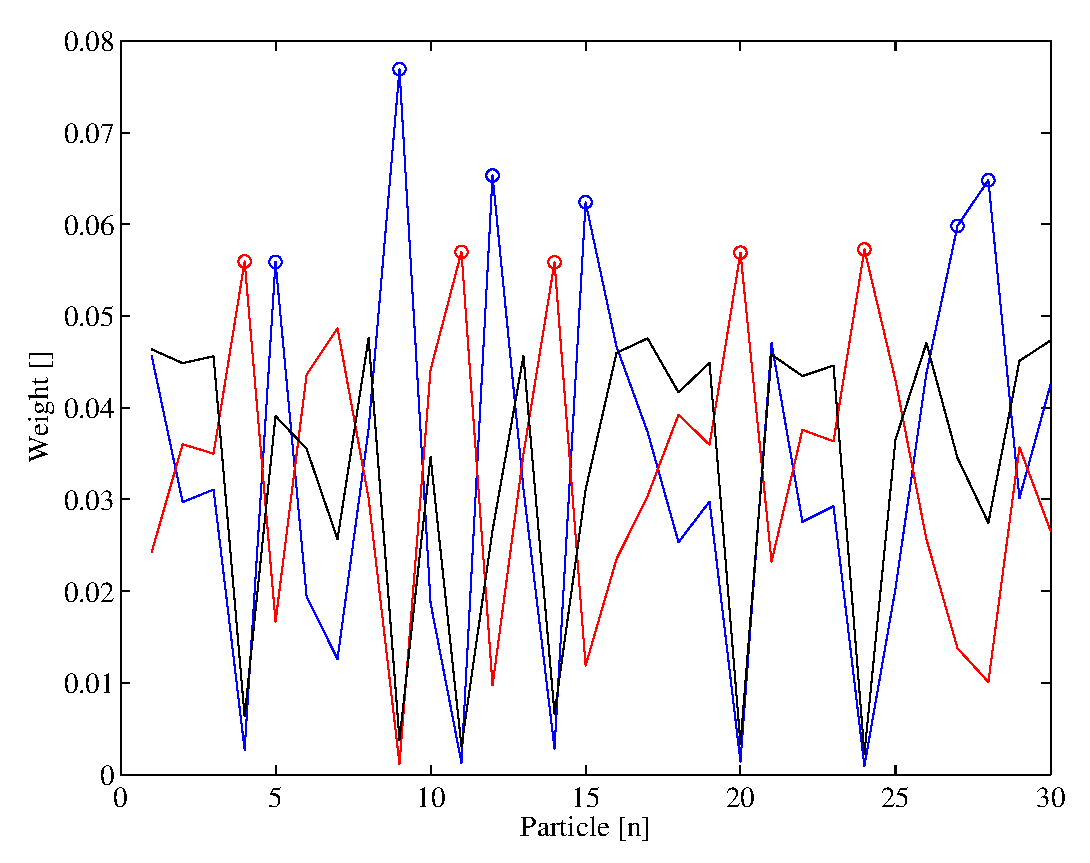
\includegraphics[width=\columnwidth]{../FinalFigures/Depletion}}
\subfigure[Forward (black) and reverse (red) model.  Simple pendulum with two different particle filters: the single particle filter that draws from  (circles), and the independent particle filters (squares).]{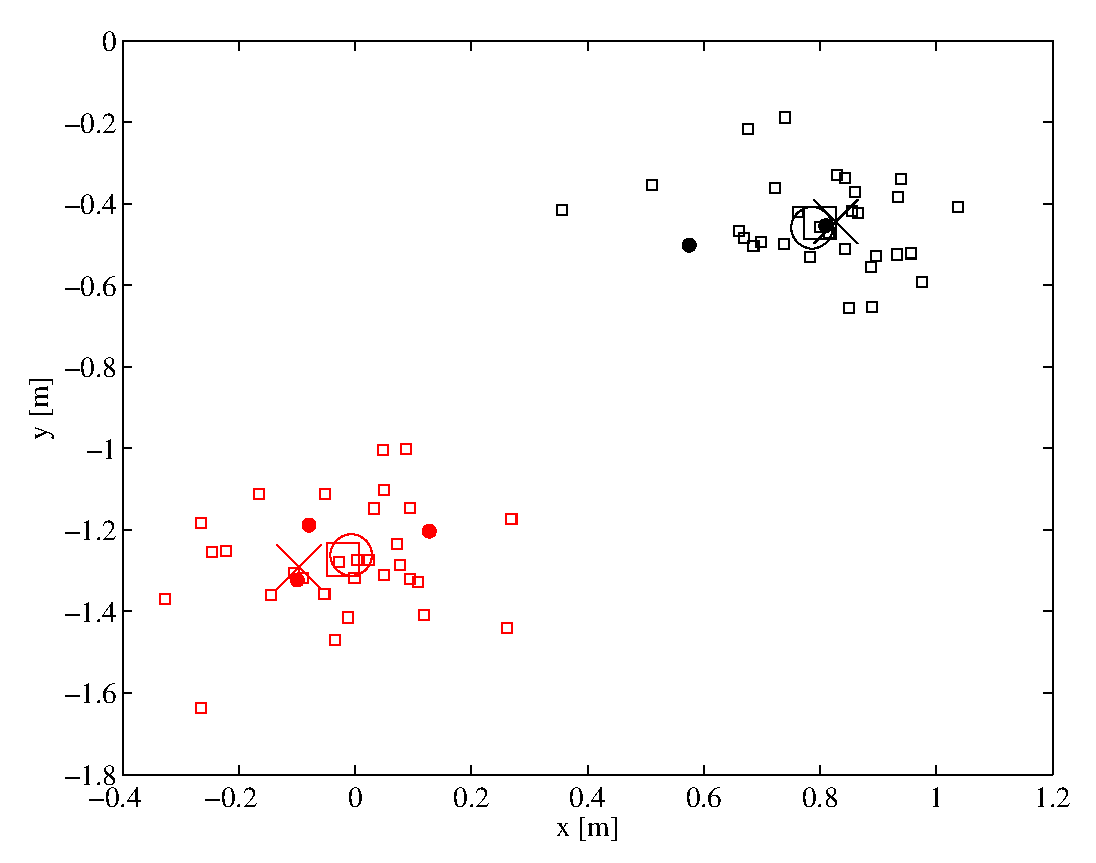
\includegraphics[width=\columnwidth]{../FinalFigures/IndependentlySampled}}
\caption{Example where the mediocre points of each set get chosen causing .}
\label{fig:deplete}
\end{figure}

While \cite{howard2006multi}